\chapter{Scene Geometry Reconstruction}
\label{ch:Scene Geometry}

\section{Finding the vanishing line $l'_\infty$ of the horizontal plane}

\begin{Procedure}[label=proc:FindingIntersection]{Robust finding of the intersection between multiple intersecting lines}
This procedure aims at finding the intersection point $P$ of a given set of $n \geq 2$ intersecting lines $l_i \, \forall i \in \{1, ..., n\}$. Both the point $P$ and the lines $l_i$ are provided in homogenous coordinates. Thus $$\underline{P} \overset{\Delta}{=} \colvec{P_x, P_y, 1}$$ and $$\underline{l_i} \overset{\Delta}{=} \colvec{l_{ix}, l_{iy}, 1} \, \forall i \in \{1, ..., n\}$$. The matrix $L$ is defined as $$L = \matrixdim{1}{4}{\underline{l_1}, \underline{l_2}, \dots, \underline{l_n}}$$

Were all the lines perfectly intersecting in a single point it would hold $$L^T\underline{P} = \underline{0}$$

and thus

$$\underline{P} \in RNS(L)$$

Unfortunately, in the real world, seldom do $n$ "intersecting" lines actually intersect. An approximated solution is needed and thus the problem becomes an optimization one:

$$
\underline{P} \overset{\Delta}{=} \argmin_{\underline{x}} ||L^T\underline{x}||_2
$$

This problem can be solved using the Singular Value Decomposition (SVD) on the $L$ matrix:
\begin{equation}
    \begin{matrix}
        L = U \Sigma V^T \\
        \text{ where } \\
        U, \Sigma, V \in \mathbb{R}^{3x3}, \\
        U\cdot U^T = I, \\
        V\cdot V^T = I,\\
        \Sigma_{ii} = \sigma_i \in \mathbb{R} \; \forall i \in \{1, ..., 3\}, \\
         \Sigma_{ij} = 0 \; \forall i \in \{1, ..., 3\}, \forall j \in \{1, ..., 3\}, i\neq j, \\
         |\sigma_i| >= |\sigma_j| \; \forall i, j \in \{1, ..., 3\}, i<j
    \end{matrix}
\end{equation}

Since the $\sigma_i$ are in absolute nonincreasing order it can be easily derived that the optimal solution up to scale is:

$$
\underline{P} \overset{\Delta}{=} V_n := \text{n-th column of V}
$$
\end{Procedure}

The image of the vanishing line $l'_\infty$ of the horizontal plane can be found as the line going through the images of two distinct vanishing points of the horizontal plane. Luckily, the vanishing point associated with a direction in the horizontal plane is shared with all parallel planes, and thus the $m$s and $l$s lines will all meet respectively in the vanishing points $v_m$ and $v_l$. 

Using Procedure~\ref{proc:FindingIntersection} the best approximation for $v_m$ and $v_l$ can be computed.

The line $l'_\infty$ is now defined as :

\begin{equation*}
\begin{split}
l'_{\infty{}}^T v_m &= 0\\
l'_{\infty{}}^T v_l &= 0
\end{split}
\end{equation*}

and thus:

$$
l'_\infty{} \overset{\Delta}{=} v_m \times v_l
$$

The results of the extraction are the following:

$$
l'_\infty{} \overset{\Delta}{=}\colvec{-8.0288 \cdot 10^{-05}, -0.0011, 1}
$$

\begin{figure}[H]
\centering
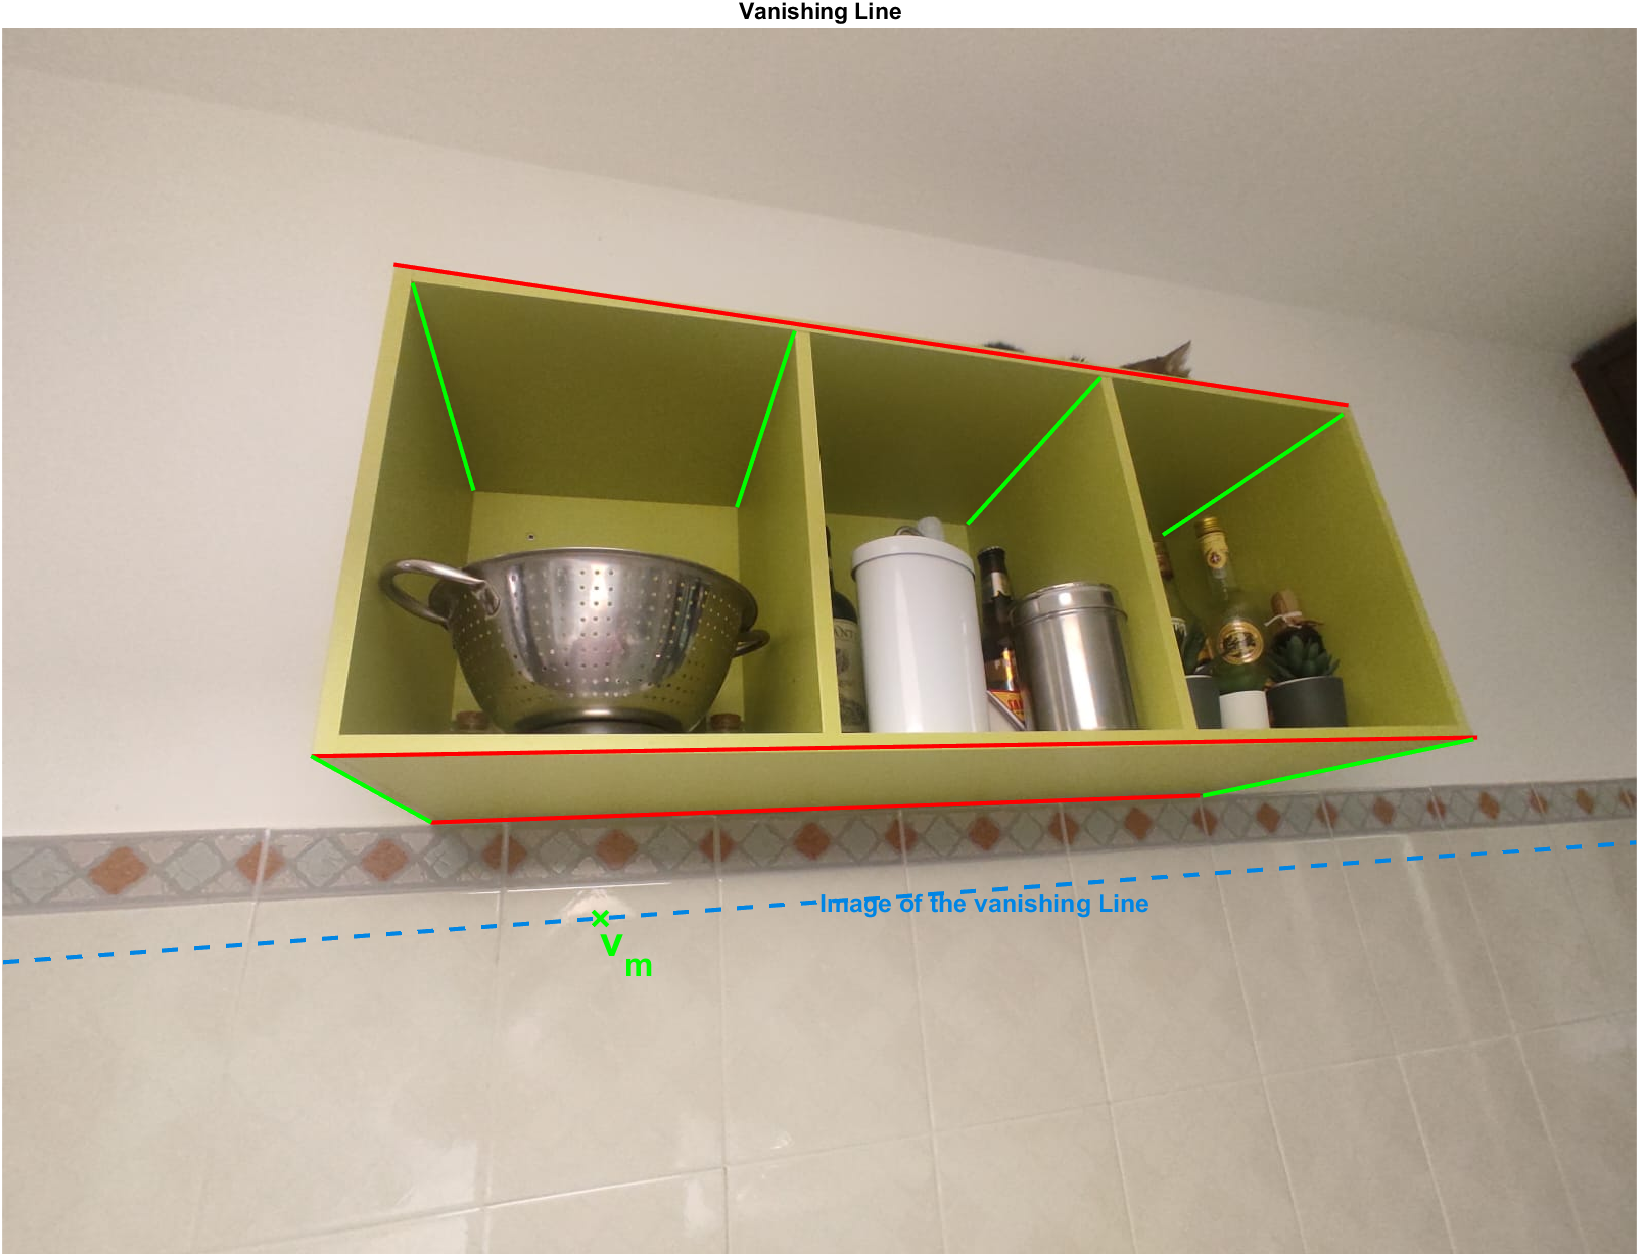
\includegraphics[height=9.5cm, width=\textwidth, keepaspectratio]{Report/Images/2.1-VanishingLine/Vanishing Line.png}
\caption{\label{fig:Vanishing Line}The Extracted image of the vanishing line}
\end{figure}


\section{Metric Rectification and depth estimation}
To rectify the upper face of the cabinet a stratified approach has been chosen. The rectification is the outcome of three steps:
\begin{enumerate}
    \item Affine Rectification
    \item Affinity to make $C$ a circle
    \item Affinity to align the axis and allign the plot (optional)
\end{enumerate}

\subsection{Affine Rectification}
The purpose of the affine rectification is to find the Homography $H_{aff}$ such that $$H_{aff}^{-T} 
 \cdot l_{\infty{}}' = l_\infty{} = \colvec{0, 0, 1}$$

 Consequently $H_{aff}$ has to be of this form:
 $$
 H_{aff} = \matrixdim{3}{3}{*, *, *, *, *, *, ,l_{\infty{}}'^T, }
 $$

 In order to make the affine reconstructed image of a more manageable size the following homography has been chosen:

  $$
 H_{aff} = \matrixdim{3}{3}{\frac{1}{10}, 0, 0, 0, \frac{1}{10}, 0,-8.0288 \cdot 10^{-05}, -0.0011, 1}
 $$

 \begin{figure}[H]
\centering
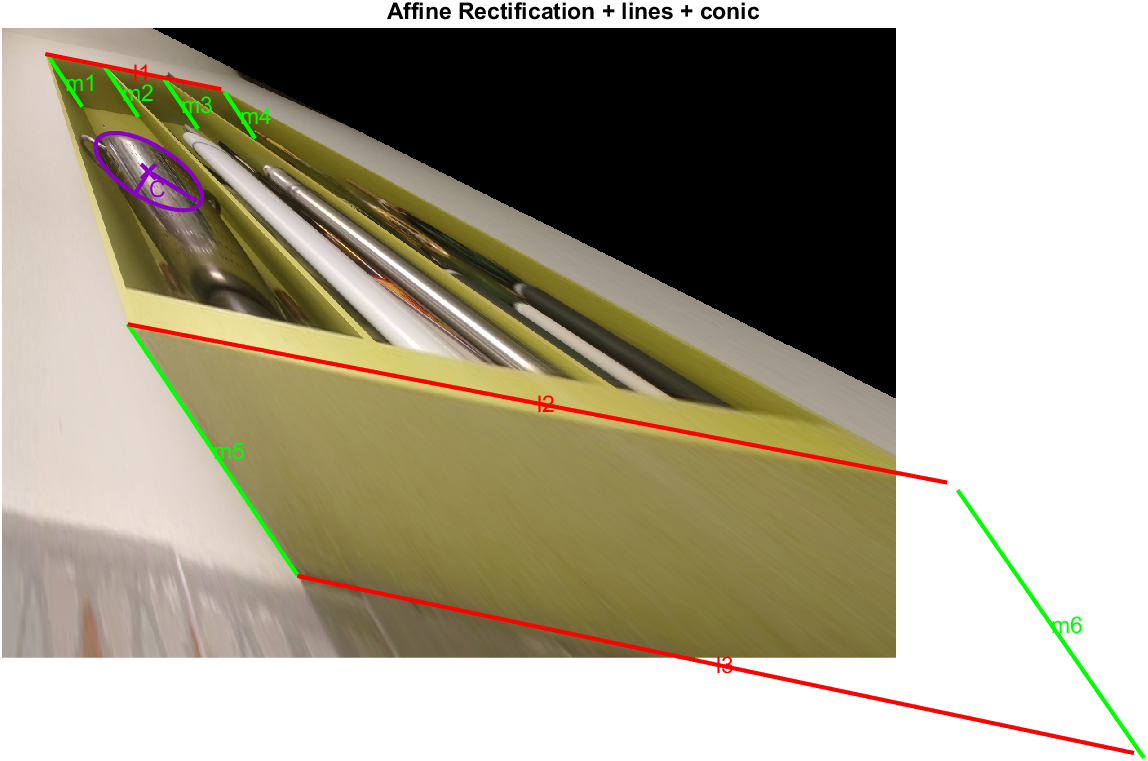
\includegraphics[height=9.5cm, width=\textwidth, keepaspectratio]{Report/Images/2.2-MetricRectification/Affine Rectification.png}
\caption{\label{fig:Affine rectification}The result of the affine rectification}
\end{figure}

\subsection{Affinity to make $C$ a circle}
Given the extracted conic $C$ in homogeneous matrix form, one can apply the affine rectification obtaining:
$$
C_{aff} = H_{aff}^{-T} \cdot C \cdot H_{aff}^{-1}
$$

From that the length ($a$ and $b$) and direction ($\theta$) of the ellipse' axis as well as the ellipse center's coordinates ($C_c$) can be extracted:

\begin{equation*}
\begin{split}
a &= 74.0106\text{ pixels}\\
b &= 31.8570\text{ pixels}\\
\theta &= 0.5529\text{ rad}\\
C_C &= \colvec{180.4210, 176.4675, 1} \text{ pixels}
\end{split}
\end{equation*}

The Homography necessary to turn $C_{aff}$ back into a circle can be factored into an isometry $U$ and a scaling $S$ as $H_{circle} = U S U^{-1}$. The two homographies can be built as follows:

\begin{equation*}
\begin{split}
U &= \matrixdim{3}{3}{\cos{\theta}, -\sin{\theta}, , \sin{\theta}, \cos{\theta}, C_c, 0, 0, }\\
S &= \matrixdim{3}{3}{1, 0, 0, 0, a/b, 0, 0, 0, 1}\\
\theta &= 0.5529\text{ rad}
\end{split}
\end{equation*}

Thus a shape reconstructing homography can be:
$$H_{metric} = H_{circle} \cdot H_{aff}$$

\subsection{Affinity to align the axis and align the plot (optional)}

To facilitate subsequent tasks another affinity is necessary to align the $l$ lines to the x-axis and to center the plot. This is encapsulated in $H_{offset}$

The final Rectifing Homography is thus:

$$H_{metric} = H_{off} \cdot H_{circle} \cdot H_{aff} = \matrixdim{3}{3}{0.1041, -0.2222, 138.2097, -0.0286, 0.1633, -14.5239, -0.0001, -0.0011, 1}$$

